\documentclass[landscape]{exam}

\usepackage{2in1, lscape} 
\usepackage{units} 
\usepackage[fleqn]{amsmath}
\usepackage{float}
\usepackage{mdwlist}
\usepackage{booktabs}
\usepackage{caption}
\usepackage{fullpage}
\usepackage{enumerate}
\usepackage{graphicx}

\printanswers

\everymath{\displaystyle}

\printanswers

\title{Statistics \\ Week Four}
\date{\today}
\author{}

\begin{document}

\maketitle
\tableofcontents

  \section{Equations of Lines}
  \begin{itemize*}
    \item Explain slope, y-intercept, etc.
    \item show how to get slope from two points
    \item show how to get equation from slope and one point
  \end{itemize*}

  \section{Halftime vs. Final}

  \begin{figure}[H]
    \centering
    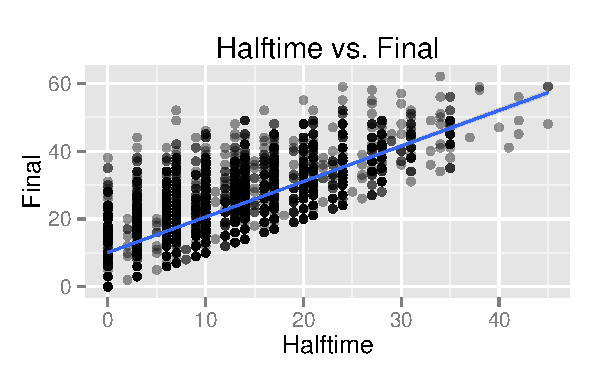
\includegraphics{figures/nfl/ht_vs_final.pdf}
    \caption{Halftime vs. Final Score}
  \end{figure}

  % \begin{figure}[H]
  %   \centering
  %   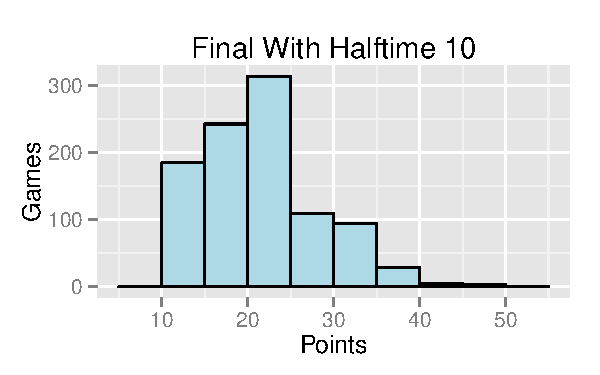
\includegraphics{figures/nfl/ht_10_final.pdf}
  %   \caption{Final score with a halftime score of 10}
  % \end{figure}

  \begin{figure}[H]
    \centering
    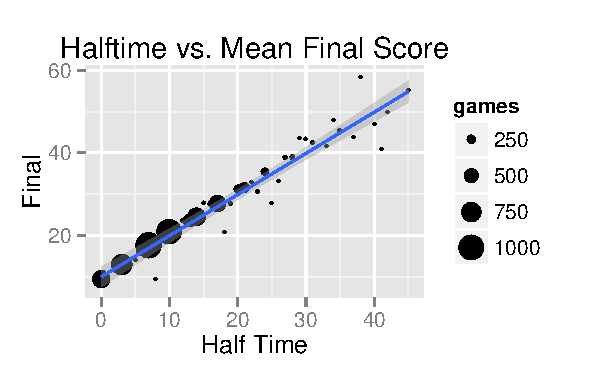
\includegraphics{figures/nfl/ht_vs_mean_final.pdf}
    \caption{Halftime vs. Mean Final Score}
  \end{figure}

  \begin{figure}[H]
    \centering
    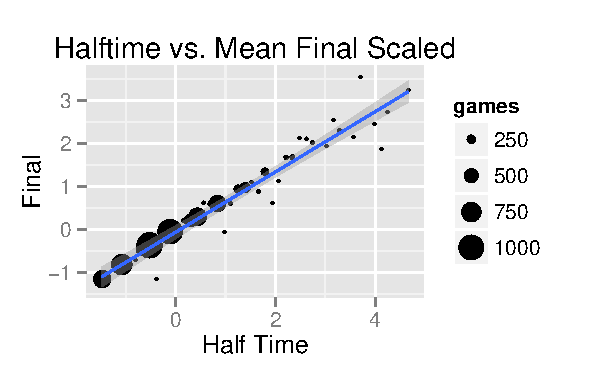
\includegraphics{figures/nfl/ht_vs_mean_final_scaled.pdf}
    \caption{Halftime vs. Mean Final (scaled)}
  \end{figure}

  \begin{table}[H]
    \centering
    \begin{tabular}{rrrrr}
      \toprule
      \midrule
      Halftime & Mean Final & Halftime s & Final s & slope\\
      0        & 9.53       & -1.48      & -1.15   & NA \\
      3        & 13.06      & -1.07      & -0.81   & 0.83 \\
      7        & 17.76      & -0.53      & -0.36   & 0.83 \\
      10       & 20.96      & -0.12      & -0.05   & 0.75 \\
      14       & 24.61      & 0.43       & 0.30    & 0.64 \\
      17       & 27.81      & 0.84       & 0.61    & 0.75 \\
      \bottomrule
    \end{tabular}
    \caption{Common halftime scores (at least 500 games)}
  \end{table}

  \begin{tabular}[H]{rrl}
    \toprule
    Min Games & Mean Slope & Notes \\
    \midrule
    500       & 0.76       & not enough samples\\
    all       & 0.84       & outliers \\
    100       & 0.73       & just right \\
    \bottomrule
  \end{tabular}

  $r = 0.7376$

  Line goes through $(0, 0)$, so the equation is:
  \[
    \hat{z}_y = r z_x
  \]

  for halftime/final scores:
  \[
    \hat{z}_y = 0.7376 z_x
  \]

  \begin{itemize*}
    \item $r$ is number of y standard deviations change for each x standard
      deviation change 

    \item $r = \pm 1$ for exact match

    \item $r = 0$ for no correlation.  If you change x, you don't expect any
      corresponding change in y

    \item minimizes square of differences from prediction
  \end{itemize*}

  Average slope of means approximately $r$.
  examples:

  \begin{tabular}[H]{rrrr}
    \toprule
    x  & $z_x$   & $\hat{z}_y$ & y \\
    \midrule
    7  & $-0.53$ & $-0.39$     & 17.4 \\
    17 & $0.84$  & $0.62$      & 27.9 \\
    \bottomrule
  \end{tabular}

  If we want things in points instead of standard deviations, we have to convert
  everything:

  slope:
  \[
    a = r \cdot \frac{s_y}{s_x}
  \]

  Line goes through $(\bar{x}, \bar{y})$.  Find y-intercept:

  \begin{align*}
    \bar{y} & = a \bar{x} + b \\
    b         & = \bar{y} - a \bar{x} \\
  \end{align*}

  \begin{tabular}[H]{lrr}
    \toprule
             & mean & standard deviation \\
    \midrule
    halftime & 10.9 & 7.4 \\
    final    & 21.5 & 10.4 \\
    \bottomrule
  \end{tabular}

  \begin{align*}
    a & = 0.7376 \cdot \frac{10.4}{7.4} \\
      & = 1.04 \\
    \\
    b & = 21.5 - 1.04 \cdot 10.9 \\
      & = 10.16 \\
    \\
    \hat{y} &= 1.04 x + 10.16 \\
  \end{align*}

  \begin{tabular}[H]{rr}
    \toprule
    halftime & predicted final \\
    \midrule
    14       & 24.8 \\
    3        & 13.2 \\
    \bottomrule
  \end{tabular}

  \section{Final vs. Halftime}

  You get a different model going the other direction.
  \begin{align*}
    a & = 0.7376 \cdot \frac{7.4}{10.4} \\
      & = 0.52 \\
    \\
    b & = 10.9 - 0.52 \cdot 21.5 \\
      & = -0.27 \\
    \\
    \hat{y} &= 0.52 x - 0.27 \\
  \end{align*}

  without rounding error:
  \[
    \hat{y} = 0.5195 - 0.3036 x +  \\
  \]

  \begin{tabular}[H]{rr}
    \toprule
    final & predicted halftime \\
    \midrule
    30    & 15.28 \\
    10    & 4.89 \\
    \bottomrule
  \end{tabular}

  \section{Examples}
  \begin{itemize}
    \item In a class, midterm and final scores have a mean of 60 and an SD of 15.
      The correlation between midterm and final scores is 0.5.  Estimate the average
      final scores for a midterm score of:

      \begin{parts}
        \part midterm: 75
          \begin{solution}
            1 SD above the mean, final should be $60 + 0.5 \cdot 15 = \boxed{ 67.5 }$
          \end{solution}

        \part midterm: 30
          \begin{solution}
            2 SD below the mean, final should be $60 - 0.5 \cdot 30 = \boxed{ 45 }$
          \end{solution}
          
        \part midterm: 60
          \begin{solution}
            at the mean.  final also 60
          \end{solution}
      \end{parts}

    \item For men age 45-54 in HANES sample:
      \begin{tabular}[H]{lrr}
               & mean   & SD \\
        height & 69 in  & 3 in \\
        weight & 171 lb & 30 lb \\
      \end{tabular}

      $r = 0.4$

      \begin{parts}
        \part what is the expected weight for a 69 inch man?
        \begin{solution}
          1 SDs above mean.  $171 + 0.4 \cdot 30 = \unit[183]{lb}$
        \end{solution}

        \part what is the expected weight for a 63 inch man?
        \begin{solution}
          2 SDs below mean.  $171 - 2 \cdot 0.4 \cdot 30 = \unit[147]{lb}$
        \end{solution}

        \part What is the general equation for the regression line?
          \begin{solution}
            \[
              \hat{y} = 0.9913 x + 102.6
            \]
          \end{solution}

        \part what is the expected weight for a 0 inch tall man?
        \begin{solution}
          102.6 lbs but you should be a little suspicious about a 0 inch tall man.
        \end{solution}

      \end{parts}

    \item For some school:
      \begin{tabular}[H]{lrr}
            & mean   & SD \\
        SAT & 550  & 80 \\
        GPA & 2.6 & 0.6 \\
      \end{tabular}

      $r = 0.4$

      What is the expected GPA for a student with an SAT score of 650?

      \begin{solution}
        \[
          z_x = \frac{650 - 550}{80} = 1.25
        \]

        1.25 SD above mean.

        \[
          \hat{z}_y = 0.4 \cdot 1.25 = 0.5
        \]

        Convert back to GPA:
        \[
          2.6 + 0.5 \cdot 0.6 = 2.9
        \]
      \end{solution}

    \item The mean age 45-54 in the HANES sample had an average height of 69
      inches.  This is the same as the overall average height.

      T/F: their average weight should be around 171 lbs (overall average weight)?

      \begin{solution}
        False.  The average weight for people 69 inches tall is the average of a
        vertical slice over 69.  This probably will about match the overall average.

        However, men 45-54 don't all appear in the vertical slice over 69.  They're
        scattered about the graph.  Older men tend to be heavier for their height, so
        the average weight of this group is probably higher than 171 lbs.
      \end{solution}

    \item In regression of height to weight, men who are 73 inches tall average 176
      lbs in weight.  T/F: men who are 176 lbs average 73 inches tall?
  \end{itemize}

  \section{Regression to the Mean}
  For any repeated test, people tend to be closer to the mean on the second attempt.

  \begin{itemize*}
    \item pilots with bad/good landings and instructor criticism/praise.
    \item retake of standardized tests
  \end{itemize*}

  \section{Error}

  \section{Outliers}

\end{document}

